\documentclass[10pt,openany,a4paper]{article}
\usepackage{amsmath, amsfonts, amssymb, amsthm}
\usepackage{tikz, pgfplots, tkz-euclide,calc}
    \usetikzlibrary{patterns,snakes,shapes.arrows}
\usepackage{fancyhdr}
\usepackage{enumerate,enumitem}
\usepackage{cancel}
\usepackage{varwidth}

% TAMBAHKAN PACKAGE SENDIRI KALAU KURANG

\usepackage{geometry}
\geometry{
	total = {160mm, 237mm},
	left = 25mm,
	right = 20mm,
	top = 30mm,
	bottom = 30mm,
}


\pagestyle{fancy}
\fancyhead{}
\fancyfoot{}
\fancyhead[r]{}
\fancyhead[l]{\fbox{\large{\textbf{SKPB - ITS}}}}
\renewcommand{\headrulewidth}{0pt}
\renewcommand{\footrulewidth}{0pt}


\begin{document}

    \begin{center}
	{\underline{\textbf{\MakeUppercase{Evaluasi Tengah Semester Bersama Genap 2021/2022}}}}
    \end{center}

    \begin{center}
	\begin{tabular}{lcl}
		Mata kuliah/SKS & : & Matematika 2 ( KM18 4 201 ) / 3 SKS\\
		Hari, Tanggal & : & Rabu, 8 Juni 2022\\
		Waktu & : & 13.30-15.10 WIB (100 menit)\\
		Sifat & : & Tertutup\\
		Kelas & : & 48-63
	\end{tabular}
    \end{center}
	
    \noindent\rule{\textwidth}{2.pt}
	
    \setlength{\parindent}{5pt}
    \par Diberikan 5 soal, dengan bobot nilai masing-masing soal sama dan boleh dikerjakan tidak berurutan.
    \setlength{\parindent}{5pt}
    \centering{Tuliskan: Nama, NRP, dan Nomor Kelas pada lembar jawaban Anda.}
    \setlength{\parindent}{5pt}
    \par \textbf{\MakeUppercase{Tidak boleh menggunakan kalkulator dan alat komunikasi}}
    \centering{\textbf{\MakeUppercase{dilarang memberikan/menerima jawaban selama ujian}}}
    \par \centering{\textbf{"Setiap tindak kecurangan akan mendapat sanksi akademik."}}
	
    \noindent\rule{\textwidth}{2.pt}
	
% SOAL DI SINI YAA
    \begin{enumerate}
	\item Tentukan semua nilai $x$ yang memenuhi
        \[1<\frac{1}{|x-2|}\leq4\]

        \item diketahui $f(x)=\frac{1+x}{1-x}$ dan $g(x)=\frac{x}{1-x}$,
        \begin{enumerate}
            \item Dapatkan domain $f$ dan $g$.
            \item Dapatkan $(f\circ g)(x)$ beserta domainnya.
        \end{enumerate}

        \item Diberikan fungsi $f(x)=x^2-2x+1$
        \begin{enumerate}
            \item Tentukan nilai $k$ terbesar sehingga $f(x)$ memiliki invers pada $[-\infty,k]$.
            \item Tentukan $f^{-1}(x)$.
            \item Sketsa grafik $f(x)$ dan $f^{-1}(x)$ dalam satu bidang koordinat.
        \end{enumerate}

        \item Diberikan fungsi $f(x)=\begin{cases}
        2|x+1|&   x < -1\\
        \\
        x^2 &   x \geq 1
        \end{cases}$
        \begin{enumerate}
            \item hitunglah $\lim\limits_{x\to-1}f(x)$.
            \item Berapa nilai $f(-1)$?
            \item Apakah $f(x)$ kontinu? jelaskan!
        \end{enumerate}
        Apakah $f(x)$ kontinu di $x=-1$? jelaskan!

        \item Diketahui garis singgung pada kurva $y^3=2x^2$ di titik $(a,b)$ sejajar dengan garis $2x+3y-5=0$. Tentukan titik $(a,b)$.
    \end{enumerate}
	
    \vspace*{2cm}
    \hrulefill\textbf{ Selamat Mengerjakan }\hrulefill

    \begin{center}
	"\textit{Jujur adalah kunci kesuksesan}"
    \end{center}

    \newpage
    \fancyhead[l]{}
    \fancyfoot[RO,RE]{\textit{By: Teosofi Hidayah Agung (5002221132)}}
    \begin{enumerate}
        \item Bagi kasus pada pertidaksamaan.
        \begin{enumerate}[label=(\arabic*)]
            \item Untuk $1<\frac{1}{|x-2|}$ diperoleh:\\
            \textit{(*Catatan: Hasil nilai mutlak selalu positif, sehingga jika kedua ruas dikali $|x-2|$ tidak akan mengubah tanda pertidaksamaan)}
            \begin{align*}
                1<\frac{1}{|x-2|}&\hspace{4.0cm}\\
                1|x-2|<1&,\quad x\neq2 \textrm{\textbf{ (Penyebut tak nol)}}\\
                |x-2|<1&,\quad x\neq2\\
                -1<x-2<1&,\quad x\neq2 \textrm{\textbf{ (Definisi jarak)}}\\
                1<x<3&,\quad x\neq2\\
            \end{align*}
            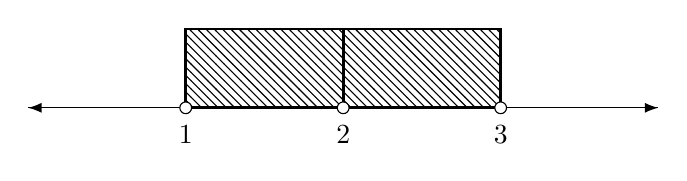
\begin{tikzpicture}
                \draw[-Latex] (0,0) -- (8,0);
                \draw[Latex-] (0,0) -- (8,0);
                \foreach \i in {1,2,3}
                {
                \coordinate (A\i) at ({2*\i},0);
                \node[below] at ($(0,-0.1)+(A\i)$) {$\i$};
                }
                
                \draw[fill=lightgray,pattern=north west lines,line width=1pt](A1)rectangle($(A2)+(0,1)$);
                \draw[fill=lightgray,pattern=north west lines,line width=1pt](A2)rectangle($(A3)+(0,1)$);
                
                \foreach \i in {1,2,3}
                \node[circle,draw,fill=white,inner sep=1.5pt] at (A\i) {};
                
            \end{tikzpicture}\\
            $HP_1=\{x\:|\:1<x<2 \:\vee\: 2<x<3\}=(1,2)\cup(2,3)$

            \item Untuk $\frac{1}{|x-2|}\leq4$ diperoleh:\\
            \begin{align*}
                \frac{1}{|x-2|}\leq4&\hspace{4.0cm}\\
                1\leq4|x-2|&,\quad x\neq2 \textrm{\textbf{ (Penyebut tak nol)}}\\
                \frac{1}{4}\leq|x-2|&,\quad x\neq2\\
                \frac{1}{4}\leq x-2\:\bigvee\:-\frac{1}{4}\geq x-2&,\quad x\neq2 \textrm{\textbf{ (Definisi jarak)}}\\
                \frac{1}{4}+2\leq x\:\bigvee\:-\frac{1}{4}+2\geq x&,\quad x\neq2\\
                \frac{9}{4}\leq x\:\bigvee\:\frac{7}{4}\geq x&,\quad x\neq2
            \end{align*}
            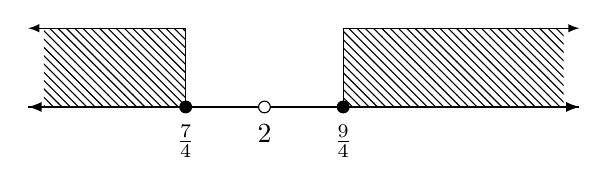
\begin{tikzpicture}
                \draw[-Latex] (-1,0) -- (6,0);
                \draw[Latex-] (-1,0) -- (6,0);
                \foreach \i in {1,2,3}
                \coordinate (A\i) at (\i,0);
                \node[below] at ($(0,-0.1)+(A1)$) {$\frac{7}{4}$};
                \node[below] at ($(0,-0.1)+(A2)$) {$2$};
                \node[below] at ($(0,-0.1)+(A3)$) {$\frac{9}{4}$};

                \fill[lightgray,pattern=north west lines,line width=1pt](A1)rectangle($(-0.8,0)+(0,1)$);
                \fill[lightgray,pattern=north west lines,line width=1pt](A3)rectangle($(5.8,0)+(0,1)$);
                
                \draw[-latex](A1)--($(A1)+(0,1)$)--($(-1,0)+(0,1)$);
                \draw[-latex](A3)--($(A3)+(0,1)$)--($(6,0)+(0,1)$);
                
                \foreach \i in {1,3}
                \node[circle,draw,fill=black,inner sep=1.5pt] at (A\i) {};
                \node[circle,draw,fill=white,inner sep=1.5pt] at (A2) {};
                
            \end{tikzpicture}\\
            $HP_2=\left\{x\:|\:x\leq\frac{7}{4} \:\vee\: x\geq\frac{9}{4}\right\}=\left(-\infty,\frac{7}{4}\right]\cup\left[\frac{9}{4},+\infty\right)$
        \end{enumerate}
        Sehingga irisan kedua himpunan penyelasaian\\~\\
        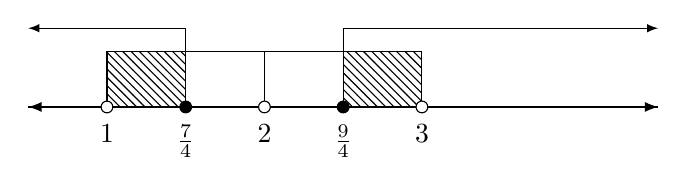
\begin{tikzpicture}
            \draw[-Latex] (0,0) -- (8,0);
            \draw[Latex-] (0,0) -- (8,0);
            \foreach \i in {1,2,3,4,5}
                \coordinate (A\i) at (\i,0);
            \node[below] at ($(0,-0.1)+(A1)$) {$1$};
            \node[below] at ($(0,-0.1)+(A2)$) {$\frac{7}{4}$};
            \node[below] at ($(0,-0.1)+(A3)$) {$2$};
            \node[below] at ($(0,-0.1)+(A4)$) {$\frac{9}{4}$};
            \node[below] at ($(0,-0.1)+(A5)$) {$3$};

            \fill[lightgray,pattern=north west lines,line width=1pt](A1)rectangle($(A2)+(0,0.7)$);
             \fill[lightgray,pattern=north west lines,line width=1pt](A4)rectangle($(A5)+(0,0.7)$);

            \draw(A1)rectangle($(A3)+(0,0.7)$);
            \draw(A3)rectangle($(A5)+(0,0.7)$);
            \draw[-latex](A2)--($(A2)+(0,1)$)--($(0,0)+(0,1)$);
            \draw[-latex](A4)--($(A4)+(0,1)$)--($(8,0)+(0,1)$);

            \foreach \i in {1,3,5}
                \node[circle,draw,fill=white,inner sep=1.5pt] at (A\i) {};
            \foreach \i in {2,4}
                 \node[circle,draw,fill=black,inner sep=1.5pt] at (A\i) {};
        \end{tikzpicture}\\
        $HP=HP_1\cap HP_2=\left\{x\:|\:1<x\leq\frac{7}{4}\:\vee\:\frac{9}{4}\leq x<3\right\}=\left(1,\frac{7}{4}\right]\cup\left[\frac{9}{4},3\right)$.
        
        \item \begin{enumerate}
            \item Karena fungsi berbentuk pecahan, maka penyebutnya tidak boleh nol.
            \begin{flalign*}
                D_f&=\{x\:|\:x\neq 1\}&\\
                D_g&=\{x\:|\:x\neq 1\}
            \end{flalign*}

            \newpage
            \fancyhead[l]{}
            \fancyfoot[RO,RE]{\textit{By: Teosofi Hidayah Agung (5002221132)}}
            \item Ingat bahwa $(f\circ g)(x)=f(g(x))$, sehingga
            \begin{flalign*}
                f(g(x))&=\frac{1+g(x)}{1-g(x)}&\\
                &=\frac{1+(\frac{x}{1-x})}{1-(\frac{x}{1-x})}\quad\quad\textrm{\textbf{$\left(\textrm{Subtitusi }g(x)=\frac{x}{1-x}\right)$}}&\\
                &=\frac{(\frac{1-x+x}{1-x})}{(\frac{1-x-x}{1-x})}&\\
                &=\frac{\frac{1-x+x}{\cancel{1-x}}}{\frac{1-x-x}{\cancel{1-x}}},\quad x\neq1&\\
                &=\frac{1}{1-2x},\quad x\neq1
            \end{flalign*}
            Definisi domain fungsi komposisi $f\circ g$ adalah $D_{f\circ g}=\{x\in D_g\:|\:g(x)\in D_f\}$.
            \begin{flalign*}
                D_{f\circ g}&=\{x\in \mathbb{R}/\{1\}\:|\:g(x)\in \mathbb{R}/\{1\}\}&\\
                &=\left\{x\in \mathbb{R}/\{1\}\:\Big|\:\underbrace{\frac{x}{1-x}\in \mathbb{R}/\{1\}}\right\}&\\
                &\fbox{$\displaystyle\frac{x}{1-x}\neq1$}\Rightarrow \fbox{$\displaystyle x\neq1-x$}\Rightarrow \fbox{$\displaystyle2x\neq1$}\Rightarrow \fbox{$\displaystyle x\neq\frac{1}{2}$}&\\
                &=\left\{x\in \mathbb{R}/\{1\}\:\Big|\:x\in \mathbb{R}\Big/\left\{\frac{1}{2}\right\}\right\}&\\
                &=\left\{x\in \mathbb{R}\Big/\left\{1,\frac{1}{2}\right\}\right\}&\\
            \end{flalign*}
            $\therefore(f\circ g)(x)=\frac{1}{1-2x}$ dan $D_{f\circ g}=\{x\:|\:x\neq1\:\vee\:x\neq\frac{1}{2}\}$
        \end{enumerate}

        \item \begin{enumerate}
            \item Perhatikan bahwa $f(x)=x^2-2x+1=(x-1)^2$. agar $f(x)$ mempunyai invers maka haruslah $f(x)$ fungsi satu-satu. Gambar grafiknya sebagai berikut:\\
            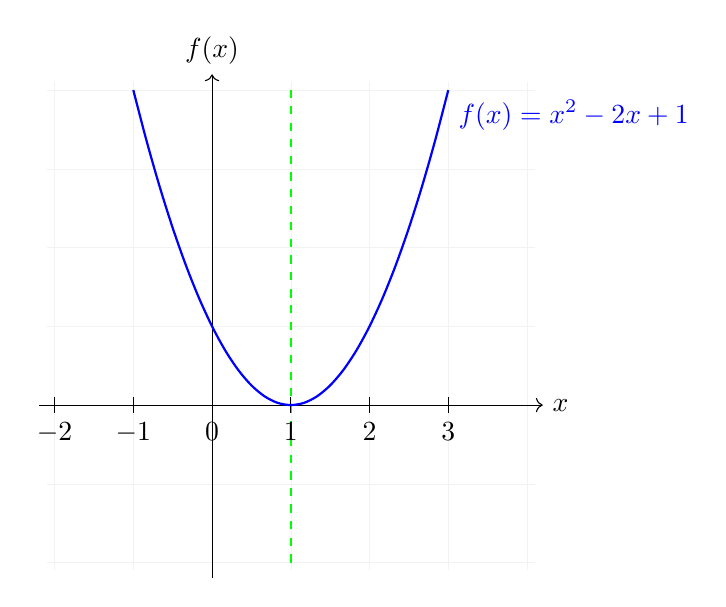
\begin{tikzpicture}
                \draw[very thin,color=lightgray!20] (-2.1,-2.1) grid (4.1,4.1);
                \draw[->] (-2.2,0) -- (4.2,0) node[right] {$x$};
                \draw[->] (0,-2.2) -- (0,4.2) node[above] {$f(x)$};
                
                \draw[thick,green,dashed,domain=-2:4,smooth]plot (1,\x);
                
                \foreach \x in {-2,-1,0,1,2,3} \draw[shift={(\x,0)},color=black] (0pt,3pt) -- (0pt,-3pt) node[below] {$\x$};
                
                \draw[thick,blue,domain=-1:3,smooth] plot (\x,{(\x-1)^2}) node [below right] {$f(x)=x^2-2x+1$};
            \end{tikzpicture}\\
            Perhatikan bahwa $f(x)$ simetri terhadap garis $x=1$. Ketika ingin mengambil $k$ terbesar agar $f(x)$ punya invers, haruslah pilih $k=1$ sehingga interval domainnya menjadi $[-\infty,1]$.\\~\\
            \textit{(*Catatan: Secara geometris suatu fungsi dikatakan punya invers ketika kita menggambar sebarang garis horizontal yang melewati grafik fungsi tersebut sedemikian sehingga hanya terdapat maksimal satu titik potong antara garis horizontal dan grafik fungsi tersebut. lebih jelasnya perhatikan gambar berikut)}\\
            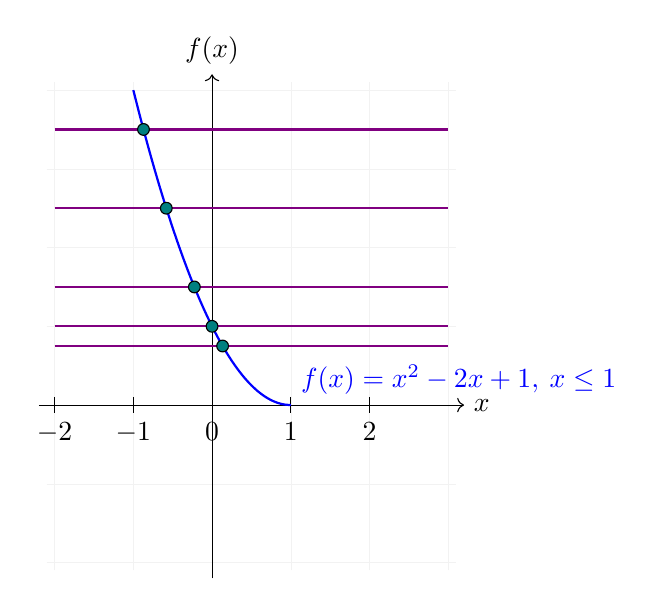
\begin{tikzpicture}
                \draw[very thin,color=lightgray!20] (-2.1,-2.1) grid (3.1,4.1);
                \draw[->] (-2.2,0) -- (3.2,0) node[right] {$x$};
                \draw[->] (0,-2.2) -- (0,4.2) node[above] {$f(x)$};
                
                \foreach \x in {-2,-1,0,1,2} \draw[shift={(\x,0)},color=black] (0pt,3pt) -- (0pt,-3pt) node[below] {$\x$};
                
                \draw[thick,blue,domain=-1:1,smooth] plot (\x,{(\x-1)^2}) node [above right] {$f(x)=x^2-2x+1,\:x\leq1$};

                \foreach \y in {3,2,1,0.5,0.25}
                {
                \draw[thick,violet,domain=-2:3,smooth]plot ({\x},{\y+0.5});
                \node[circle,draw,fill=teal,inner sep=1.5pt] at ({-sqrt(\y+0.5)+1},{\y+0.5}) {};
                }
            \end{tikzpicture}\\
            
            \item Gantikan $y$ dengan $x$ dan juga sebaliknya.
            \begin{flalign*}
                x&=(y-1)^2&\\
                x&=(y-1)^2&\\
                \sqrt{x}&=\sqrt{y-1)^2}&\\
                \sqrt{x}&=|y-1|&\\
                \pm\sqrt{x}&=y-1&\\
                y&=1\pm\sqrt{x}&\\
                f^{-1}(x)&=1\pm\sqrt{x}&\\
            \end{flalign*}
            \fancyhead[l]{}
            \fancyfoot[RO,RE]{\textit{By: Teosofi Hidayah Agung (5002221132)}}
            Karena range $R_{f^{-1}}=D_f=[-\infty,1]$, maka $f^{-1}(x)=1-\sqrt{x}$.\\~\\

            \item Salah satu cara menggambar grafik $f^{-1}(x)$ adalah dengan mencerminkan $f(x)$ terhadap garis $y=x$, sehingga akan didapat grafik $f^{-1}(x)$.\\
            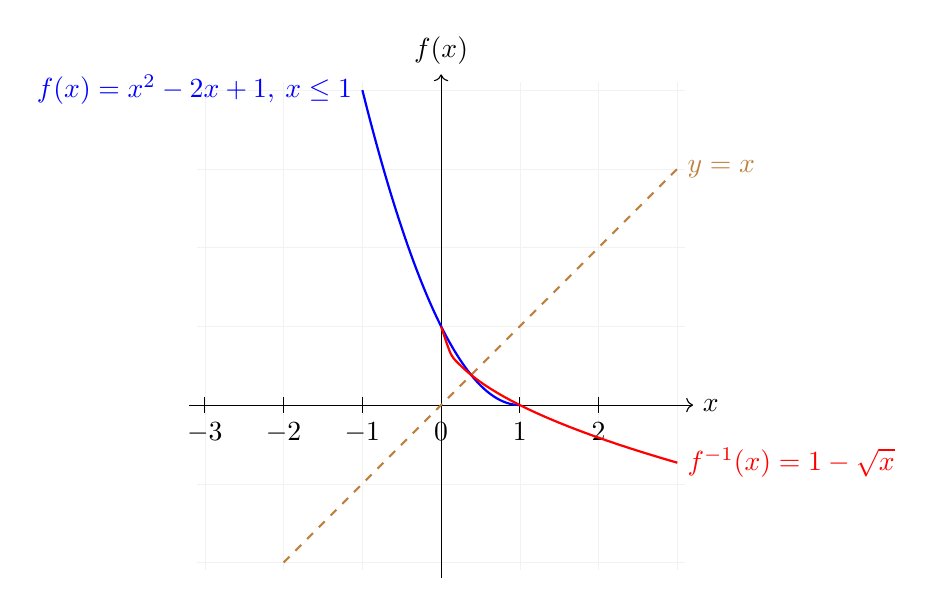
\begin{tikzpicture}
                \draw[very thin,color=lightgray!20] (-3.1,-2.1) grid (3.1,4.1);
                \draw[->] (-3.2,0) -- (3.2,0) node[right] {$x$};
                \draw[->] (0,-2.2) -- (0,4.2) node[above] {$f(x)$};
                
                \foreach \x in {-3,-2,-1,0,1,2} \draw[shift={(\x,0)},color=black] (0pt,3pt) -- (0pt,-3pt) node[below] {$\x$};

                \draw[thick,brown,dashed,domain=-2:3,smooth] plot (\x,\x) node [right] {$y=x$};
                \draw[thick,blue,domain=1:-1,smooth] plot (\x,{(\x-1)^2}) node [left] {$f(x)=x^2-2x+1,\:x\leq1$};
                \draw[thick,red,domain=0:3,smooth] plot (\x,{1-sqrt(\x)}) node [right] {$f^{-1}(x)=1-\sqrt{x}$};

            \end{tikzpicture}\\
            \end{enumerate}
            
            \item Secara definisi $f(x)=\begin{cases}
        2|x+1|&   x < -1\begin{cases}
            2x+2&\quad x>=-1,x<-1\\
             -2x-2&\quad x<-1,x<-1
        \end{cases}\\
        \\
        x^2 &   x \geq -1
        \end{cases}$\\
        Perhatikan bahwa $(-\infty,-1)\cap[-1,+\infty)=\varnothing$, sehingga\\
        $f(x)=\begin{cases}
        2|x+1|&   x < -1\begin{cases}
            2x+2&\quad \varnothing\\
             -2x-2&\quad x<-1
        \end{cases}\\
        \\
        x^2 &   x \geq ‐1
        \end{cases}$\\~\\
        Dan dapat disederhanakan menjadi\\
        \fancyhead[l]{}
        \fancyfoot[RO,RE]{\textit{By: Teosofi Hidayah Agung (5002221132)}}
        $f(x)=\begin{cases}
        -2x-2&   x < -1\\
        \\
        x^2 &   x \geq -1
        \end{cases}$
        \begin{enumerate}
            \item $\lim\limits_{x\to-1}f(x)=\begin{cases}
                    \lim\limits_{x\to-1^-}f(x)=\lim\limits_{x\to-1^-}-2x-2=0\\
                    \lim\limits_{x\to-1^+}f(x)=\lim\limits_{x\to-1^-}x^2=1
                \end{cases}$\\~\\
                Karena $\lim\limits_{x\to-1^-}f(x)\neq\lim\limits_{x\to-1^+}f(x)$, maka $\lim\limits_{x\to-1}f(x)$ tidak ada.\\

            \item $f(-1)=(-1)^2=1$\\
            
            \item $f(x)$ kontinu di titik $x=a$, jika memenuhi ketiga syarat:
            \begin{itemize}
                \item $f(a)$ terdefinisi.
                \item $\lim\limits_{x\to a}f(x)$ ada.
                \item $f(a)=\lim\limits_{x\to a}f(x)$
            \end{itemize}
            $f(x)$ tidak kontinu dimana-mana karena ada titik dimana $f(x)$ tidak kontinu, yaitu di $x=-1$. 
        \end{enumerate}
        $f(x)$ tidak kontinu di $x=-1$, karena pada soal (a) sudah disebutkan bahwa $\lim\limits_{x\to-1}f(x)$ tidak ada. Hal tersebut mengakibatkan syarat kedua dari $f(x)$ kontinu tidak terpenuhi.\\~\\
        
        \item Ingat bahwa $m_s=\frac{dy}{dx}$ dengan $m_s$ adalah garis singgung fungsi $y=f(x)$. Dengan turunan implisit akan didapatkan:
        \begin{flalign*}
            \frac{d}{dx}(y^3)&=\frac{d}{dx}(2x^2)&\\
            3y^2\frac{dy}{dx}&=4x&\\
            m_s&=\frac{dy}{dx}=\frac{4x}{3y^2},\quad y\neq0
        \end{flalign*}
        Karena garis singgung melewati $(a,b)$, maka $m_s=\frac{dy}{dx}\Big|_{\tiny{\begin{matrix}x=a\\y=b\end{matrix}}}=\frac{4a}{3b^2}$. Diketahui bahwa garis singgung sejajar dengan garis $l:=2x+3y-5=0$.
        \begin{flalign*}
            2x&+3y-5=0&\\
            3y&=-2x+5&\\
            y&=\underbrace{-\frac{2}{3}}_{m_l}x+\underbrace{\frac{5}{3}}_{c}\quad \left(\textrm{Bentuk \fbox{$y=m_lx+c$}}\right)
        \end{flalign*}
        Karena garis saling sejajar, maka
        \begin{flalign*}
            m_s&=m_l&\\
            \frac{4a}{\cancel{3}b^2}&=-\frac{2}{\cancel{3}}&\\
            4a&=-2b^2&\\
            a&=-\frac{1}{2}b^2...........(1)
        \end{flalign*}
        Ingat bahwa titik $(a,b)$ juga terletak pada $y^3=2x^2$, sehingga
        \begin{flalign*}
            (b)^3&=2(a)^2&\\
            b^3&=2a^2...........(2)
        \end{flalign*}
        \fancyhead[l]{}
        \fancyfoot[RO,RE]{\textit{By: Teosofi Hidayah Agung (5002221132)}}
        Subtitusi persamaan $(1)$ ke persamaan $(2)$.
        \begin{flalign*}
            b^3&=2(-\frac{1}{2}b^2)^2&\\
            b^3&=\frac{1}{2}b^4&\\
            b^3-\frac{1}{2}b^4&=0&\\
            b^3(1-\frac{1}{2}b)&=0
        \end{flalign*}
        Didapatkan $b=0\:\vee\:b=2$. Subtitusi hasil tersebut ke persamaan $(1)$ atau $(2)$, sehingga didapat titik $(a,b)$ adalah $(0,0)$ dan $(-2,2)$. Namun karena $y\neq0$ maka satu-satunya $(a,b)$ yang memenuhi adalah $(-2,2)$.\\~\\~\\~\\

        \fancyfoot[CO,RE]{To: Dean A. Smith}
    \end{enumerate}
\end{document}